\documentclass[12pt]{article}

\usepackage[margin=.8in,letterpaper]{geometry}
\usepackage{enumitem}
\usepackage{graphicx}
\usepackage{tikz}%,graphicx,wrapfig}
\usepackage{mathpazo}
\usepackage[scaled]{helvet}
\usepackage{siunitx}
\usepackage{multicol}

\usetikzlibrary{decorations.pathmorphing,patterns}

\sisetup{number-math-rm=\mathnormal}

\renewcommand{\familydefault}{\sfdefault}

\newcommand{\pic}[2]{\includegraphics[width=#1\textwidth]{#2}}
\newcommand{\magdir}[2]{$#1\;[\mathrm{#2}]$}
\newcommand{\mb}[1]{\mathbf{#1}}

\begin{document}

\begin{center}
  Student \#: \underline{\hspace{1in}}\hspace{1.9in}
  Student Name: \underline{\hspace{2in}}\\
  \vspace{0.3in}
  {\LARGE AP Physics \hspace{0.68in} Class 8: Universal Gravitation}
\end{center}

\noindent The questions in this homework assignment cover AP 1 and C exams.

\begin{enumerate}[leftmargin=50pt,label=\underline{\hspace{0.4in}} \arabic*.]

\item A car moves in a horizontal circle with a radius of \SI{10}{m}. The
  tangential velocity of the car is \SI{30}{m/s}. What is the car's
  acceleration?
  \begin{enumerate}[noitemsep,topsep=0pt,leftmargin=18pt]
  \item\SI{3  }{m/s^2} toward the center
  \item\SI{3  }{m/s^2} away from the center
  \item\SI{90 }{m/s^2} toward the center
  \item\SI{90 }{m/s^2} away from the center
  \item\SI{270}{m/s^2} toward the center
  \end{enumerate}
  
\item A satellite orbits the Earth at a distance of \SI{100}{km}. The mass of
  the satellite is \SI{100}{kg}, while the mass of the Earth is approximately
  \SI{6.0e24}{kg}. The radius of the Earth is approximately \SI{6.4e6}{m}. What
  is the approximate force of gravity acting on the satellite?
  \begin{enumerate}[noitemsep,topsep=0pt,leftmargin=18pt]
  \item\SI{4e4}{N}
  \item\SI{6.2e6}{N}
  \item\SI{4e8}{N}
  \item\SI{6.2e9}{N}
  \item\SI{4e14}{N}
  \end{enumerate}

\item Two satellites of equal mass orbit a planet. Satellite B orbits at twice
  the orbital radius of Satellite A. Which of the following statements is
  true?
  \begin{enumerate}[noitemsep,topsep=0pt,leftmargin=18pt]
  \item The gravitational force on Satellite A is four times less than that on
    Satellite B.
  \item The gravitational force on Satellite A is two times less than that on
    Satellite B.
  \item The gravitational force on the satellites is equal.
  \item The gravitational force on Satellite A is two times greater than that
    on Satellite B.
  \item The gravitational force on Satellite A is four times greater than that
    on Satellite B.
  \end{enumerate}
  
\item A \SI{70}{kg} astronaut floats at a distance of \SI{10}{m} from a
  \SI{50000}{kg} spacecraft. What is the force of attraction between the
  astronaut and spacecraft?
  \begin{enumerate}[noitemsep,topsep=0pt,leftmargin=18pt]
  \item\SI{2.4e-6}{N}
  \item\SI{2.4e-5}{N}
  \item Zero; there is no gravity in space.
  \item\SI{2.4e5}{N}
  \item\SI{2.4e6}{N}
  \end{enumerate}
  
\item The centripetal acceleration on \SI{1,000}{kg} car in a turn is
  \SI{1e5}{m/s^2}. The radius of the turn is \SI{10}{m}. What is the car's
  speed?
  \begin{enumerate}[noitemsep,topsep=0pt,leftmargin=18pt]
  \item\SI{1e1}{m/s}
  \item\SI{1e2}{m/s}
  \item\SI{1e3}{m/s}
  \item\SI{1e4}{m/s}
  \item\SI{1e5}{m/s}
  \end{enumerate}
  
\item A proposed ``space elevator'' can lift a \SI{1,000}{kg} payload to an
  orbit of \SI{150}{km} above the Earth's surface. The radius of the Earth is
  \SI{6.4e6}{m}, and the Earth's mass is \SI{6e24}{kg}. What is the
  gravitational potential energy of the payload when it reaches orbit?
  \begin{enumerate}[noitemsep,topsep=0pt,leftmargin=18pt]
  \item\SI{1.0e3}{J}
  \item\SI{2.7e6}{J}
  \item\SI{6.1e10}{J}
  \item\SI{2.7e12}{J}
  \item\SI{1.0e15}{J}
  \end{enumerate}

\item The Earth is at an average distance of \SI{1}{AU} from the Sun and has an
  orbital period of \SI{1}{year}. Jupiter orbits the Sun at approximately
  \SI{5}{AU}. About how long is the orbital period of Jupiter?
  \begin{enumerate}[noitemsep,topsep=0pt,leftmargin=18pt]
  \item\SI{1}{year}
  \item\SI{2}{years}
  \item\SI{5}{years}
  \item\SI{11}{years}
  \item\SI{125}{years}
  \end{enumerate}
  
\item A satellite orbits the Earth at a distance of \SI{200}{km}. If the mass
  of the Earth is \SI{6.0e24}{kg} and the Earth's radius is \SI{6.4e6}{m}, what
  is the satellite's speed?
  \begin{enumerate}[noitemsep,topsep=0pt,leftmargin=18pt]
  \item\SI{1e3}{m/s}
  \item\SI{3.5e3}{m/s}
  \item\SI{7.8e3}{m/s}
  \item\SI{5e6}{m/s}
  \item\SI{6.1e7}{m/s}
  \end{enumerate}
  
\item Mars orbits the Sun at a distance of \SI{2.3e11}{m}. The mass of the Sun
  is \SI{2e30}{kg}, and the mass of Mars is \SI{6.4e23}{kg}. Approximately
  what is the gravitational force that the Sun exerts on Mars?
  \begin{enumerate}[noitemsep,topsep=0pt,leftmargin=18pt]
  \item\SI{1.6e20}{N}
  \item\SI{1.6e21}{N}
  \item\SI{3.7e21}{N}
  \item\SI{3.7e32}{N}
  \item\SI{3.7e42}{N}
  \end{enumerate}

\item When climbing from sea level to the top of Mount Everest, a hiker
  changes elevation by \SI{8848}{m}. By what percentage will the
  gravitational field of the Earth change during the climb? (The Earth's
  mass is \SI{6.0e24}{kg}, and its radius is \SI{6.4e6}{m}.)
  \begin{enumerate}[noitemsep,topsep=0pt,leftmargin=18pt]
  \item It will increase by approximately $0.3\%$.
  \item It will decrease by approximately $0.3\%$.
  \item It will increase by approximately $12\%$.
  \item It will decrease by approximately $12\%$.
  \item The gravitational field strength will not change.
  \end{enumerate}
  \newpage
  
\item Four planets, A through D, orbit the same star. The relative masses and
  distances from the star for each planet are shown in the table. For
  example, Planet A has twice the mass of Planet B, and Planet D has
  three times the orbital radius of Planet A. Which planet has the highest
  gravitational attraction to the star?
  \begin{center}
    \begin{tabular}{lll}
      \hline
      \textbf{Planet} & \textbf{Relative mass} & \textbf{Relative distance}\\
      \hline
      A\hspace{0.4in}& $2m$   & $r$    \\ \hline
      B & $m$    & $0.1r$\hspace{0.25in} \\ \hline
      C & $0.5m$\hspace{0.25in} & $2r$   \\ \hline
      D & $4m$   & $3r$   \\ \hline
    \end{tabular}
  \end{center}
  \begin{enumerate}[noitemsep,topsep=0pt,leftmargin=18pt]
  \item Planet A
  \item Planet B
  \item Planet C
  \item Planet D
  \item All have the same gravitational attraction to the star.
  \end{enumerate}

\item A satellite orbits the Earth at a distance that is four times the radius
  of the Earth. If the acceleration due to gravity near the surface of the Earth
  is $g$, the acceleration of the satellite is most nearly
  \begin{enumerate}[noitemsep,topsep=0pt,leftmargin=18pt]
  \item zero
  \item $g/2$
  \item $g/4$
  \item $g/8$
  \item $g/16$
  \end{enumerate}

\item The mass of a planet is $1⁄4$ that of Earth and its radius is half of
  Earth's radius. The acceleration due to gravity on this planet is most nearly
  \begin{enumerate}[noitemsep,topsep=0pt,leftmargin=18pt]
  \item\SI{2 }{m/s^2}
  \item\SI{4 }{m/s^2}
  \item\SI{5 }{m/s^2}
  \item\SI{10}{m/s^2}
  \item\SI{20}{m/s^2}
  \end{enumerate}
  \begin{center}
    \vspace{-.25in}
    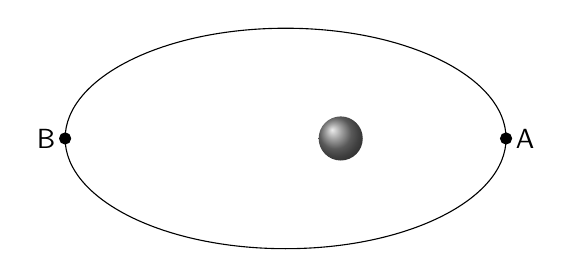
\begin{tikzpicture}[scale=1.4]
      \tikzstyle{balloon}=[ball color=gray];
      \draw(0,0) ellipse (2 and 1);
      \draw[fill=black](2,0) circle(0.05) node[right]{A};
      \draw[fill=black](-2,0) circle(0.05) node[left]{B};
      \shade[balloon] (0.5,0) circle (0.2);
    \end{tikzpicture}
  \end{center}
  
\item A satellite orbits the Earth in an elliptical orbit, with point A being
  close to the Earth and point B farther away. As the satellite moves from
  point A to point B, which of the following is true of the angularmomentum and
  kinetic energy of the satellite?
  
  \begin{tabular}{lll}
    & \underline{Angular momentum} & \underline{Kinetic energy}\\
    (a) & Increases & Remains constant \\
    (b) & Remains constant & Increases \\
    (c) & Decreases & Remains constant \\
    (d) & Remains constant & Decreases \\
    (e) & Remains constant & Remains constant
  \end{tabular}

\item Two planets of mass $M$ and $9M$ are in the same solar system. The
  radius of the planet of mass $M$ is $R$. In order for the acceleration due to
  gravity to be the same for each planet, the radius of the planet of mass
  $9M$ would have to be
  \begin{enumerate}[noitemsep,topsep=0pt,leftmargin=18pt]
  \item $1/2\;R$
  \item $R$
  \item $2R$
  \item $3R$
  \item $9R$
  \end{enumerate}
  \vspace{-0.5in}
  \begin{center}
    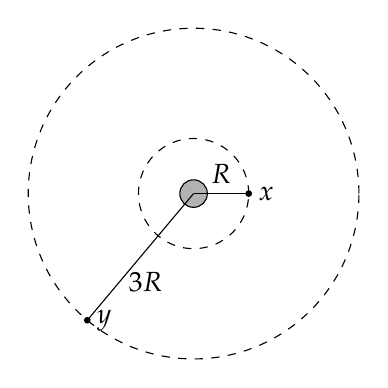
\begin{tikzpicture}[scale=0.7]
      \draw[fill=gray!60](0,0) circle(0.25);
      \draw[dashed](0,0) circle(1);
      \draw[dashed](0,0) circle(3);
      \draw(0,0)--(1,0) node[pos=1,right]{$x$} node[midway,above]{$R$};
      \draw[fill=black](1,0) circle(0.05);
      \begin{scope}[rotate=230]
        \draw(0,0)--(3,0) node[pos=1,right]{$y$} node[pos=0.7,right]{$3R$};
        \draw[fill=black](3,0) circle(0.05);
      \end{scope}
    \end{tikzpicture}
  \end{center}
\item Two planets, X and Y, orbit a star. Planet X orbits at a radius $R$, and
  Planet Y orbits at a radius $3R$. Which of the following best represents
  the relationship between the acceleration $a_X$ of Planet X and the
  acceleration $a_Y$ of Planet Y?
  \begin{enumerate}[noitemsep,topsep=0pt,leftmargin=18pt]  
  \item $a_X = 9a_Y$
  \item $9a_X = a_Y$
  \item $a_X = 3a_Y$
  \item $3a_X = a_Y$
  \item $a_X = a_Y$
  \end{enumerate}
\item A satellite is in a stable circular orbit around the Earth at a radius $R$
  and speed $v$. At what radius would the satellite travel in a stable orbit
  with a speed $2v$?
  \begin{enumerate}[noitemsep,topsep=0pt,leftmargin=18pt]  
  \item $1⁄4\;R$
  \item $1⁄2\;R$
  \item $R$
  \item $2R$
  \item $4R$
  \end{enumerate}

\item The Earth and the moon apply a gravitational force to each other.
  Which of the following statements is true?
  \begin{enumerate}[noitemsep,topsep=0pt,leftmargin=18pt]  
  \item The Earth applies a greater force on the moon than the moon exerts on
    the Earth.
  \item The Earth applies a smaller force on the moon than the moon exerts on
    the Earth.
  \item The Earth applies a force on the moon, but the moon does not exert a
    force on the Earth.
  \item The Earth does not apply a force on the moon, but the moon exerts a
    force on the Earth.
  \item The force the Earth applies to the moon is equal and opposite to the
    force the moon applies to the Earth.
  \end{enumerate}
  \newpage
  
\item Two masses exert a gravitational force $F$ on each other. If one of the
  masses is doubled, and the distance between the masses is tripled, the
  new force between them is
  \begin{enumerate}[noitemsep,topsep=0pt,leftmargin=18pt]  
  \item $6F$
  \item $2/3\;F$
  \item $2/9\;F$
  \item $3/2\;F$
  \item $4/9\;F$
  \end{enumerate}

\item A planet orbits at a radius $R$ around a star of mass $M$. The period of
  orbit of the planet is
  \begin{enumerate}[noitemsep,topsep=0pt,leftmargin=18pt]  
  \item$\displaystyle\sqrt{\frac{4\pi^2R^2}{GM}}$
  \item$\displaystyle\frac{4\pi^2R^3}{GM}$
  \item$\displaystyle\sqrt{\frac{4\pi^2R^3}{GM}}$
  \item$\displaystyle\sqrt{\frac{4\pi^2R}{GM}}$
  \item$\displaystyle\frac{GM}{4\pi^2R}$
  \end{enumerate}
  
\item A moon orbits a large planet in an elliptical orbit, with its closest
  approach at a distance $a$, and its farthest distance $b$. The speed of the
  moon at point b is $v$. The speed at point $a$ is
  \begin{enumerate}[noitemsep,topsep=0pt,leftmargin=18pt]  
  \item$\displaystyle\frac{av}{b}$
  \item$\displaystyle\frac{bv}{a}$
  \item$\displaystyle\frac{(a+b)v}{b}$
  \item$\displaystyle\frac{(b-a)v}{b}$
  \item$\displaystyle\frac{2bv}{a}$
  \end{enumerate}


\item A satellite orbits the Earth in an elliptical orbit. Which of the
  following statements is true?
  \begin{enumerate}[noitemsep,topsep=0pt,leftmargin=18pt]  
  \item The angular velocity of the satellite increases as it travels
    farther from the Earth.
  \item The acceleration of the satellite increases as it travels closer
    to the Earth.
  \item The angular momentum of the satellite increases as it travels
    closer to the Earth.
  \item The potential energy of the satellite is equal to its kinetic
    energy at all points in the orbit.
  \item The speed of the satellite must remain constant for it to remain
    in orbit around the Earth.
  \end{enumerate}

  \begin{center}
    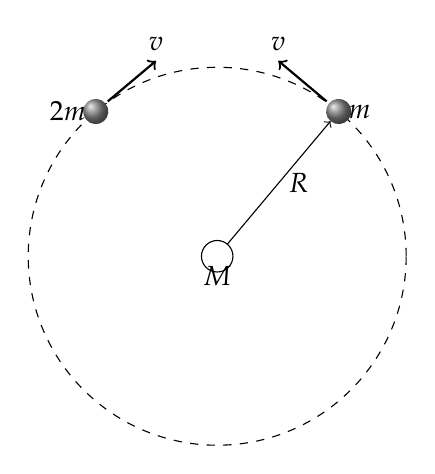
\begin{tikzpicture}[scale=0.8]
      \tikzstyle{balloon}=[ball color=gray];
      \draw(0,0) circle(0.25);
      \draw[dashed](0,0) circle(3) node[below]{$M$};
      \begin{scope}[rotate=50]
        \draw[->](0.25,0)--(2.8,0) node[midway,right]{$R$};
        \shade[balloon] (3,0) circle (0.2) node[right]{$m$};
        \draw[thick,->](3,0.25)--(3,1.25) node[pos=1,above]{$v$};
      \end{scope}
      \begin{scope}[rotate=130]
        \shade[balloon] (3,0) circle (0.2) node[left]{$2m$};
        \draw[thick,->](3,-0.25)--(3,-1.25) node[pos=1,above]{$v$};
      \end{scope}
    \end{tikzpicture}
  \end{center}
  
\item\vspace{-.2in}Two moons of mass $m$ and $2m$ orbit a planet of mass $M$ at the same
  radius $R$ and speed $v$ toward each other, as shown. The moons collide
  and stick together without destroying either moon. The total momentum of
  the moons after the collision is
  \begin{enumerate}[noitemsep,topsep=0pt,leftmargin=18pt]  
  \item $mv$
  \item $2mv$
  \item $3mv$
  \item $6mv$
  \item zero
  \end{enumerate}

\item The velocity of the two masses after the collision above is
  \begin{enumerate}[noitemsep,topsep=0pt,leftmargin=18pt]  
  \item $v$ counterclockwise
  \item $v/2$ counterclockwise
  \item $v/2$ clockwise
  \item $v/3$ counterclockwise
  \item $v/3$ clockwise
  \end{enumerate}

\item Consider a two-star system shown above, which consists of two stars of
  mass $m$ rotating in a circle of radius $r$ about their center of mass. What
  is the total energy of the two-star system?
  \begin{enumerate}[noitemsep,topsep=0pt,leftmargin=18pt]  
  \item $-Gm^2/2r$
  \item $Gm^2/2r$
  \item $Gm^2/4r$
  \item $3Gm^2/4r$
  \item $-Gm^2/4r$
  \end{enumerate}

\item If a planet has twice the radius of Earth and half of Earth's density,
  what is the acceleration due to gravity on the surface of the planet (in
  terms of the gravitational acceleration $g$ on the surface of Earth)?
  \begin{enumerate}[noitemsep,topsep=0pt,leftmargin=18pt]  
  \item $4g$
  \item $2g$
  \item $g$
  \item $g/2$
  \item $g/4$
  \end{enumerate}
\end{enumerate}

\newpage
\noindent\textbf{Free-Response Questions:}

\begin{enumerate}[leftmargin=15pt]

\item A spacecraft moving with an initial velocity $\mb{v}_0$, shown below,
  ``slingshots'' arount the sun in order to reverse its direction. The sun's
  mass is $m_\mathrm{sun}$ and you can make the assumption that the sun remains
  stationary.\\
  \begin{minipage}{0.28\textwidth}
    \pic{1.25}{shuttle.jpg}
  \end{minipage}
  \begin{minipage}{0.7\textwidth}
    \begin{enumerate}[noitemsep]
    \item What is the minimum initial speed required by the spacecraft to escape
      the sun's gravitational field and move in a trajectory toward infinity?
    \item What is the minimum initial speed $v_o$ that the spacecraft must have
      in order to avoid falling into the sun? (Treat the sun and the spacecraft
      as points.)
    \item Repeat the previous questions, but now the sun has a radius $R$.
    \item Write down the equations required to calculate the initial angle
      $\theta$ in terms of $v_0$ $d$ $m_\mathrm{sun}$, $G$ and $r$.
    \end{enumerate}
  \end{minipage}
  \newpage
\item A planet of mass $M$, radius $R$, and uniform density has a small tunnel
  drilled through the center of the planet, as shown below. When the mass is
  inside the tunnel, it experiences a force of $F=(GmM/R^3)r$, whereas when the
  mass is outside of the planet, it experiences a gravitational force of
  $F=GmM/r^2$.
  \begin{center}
    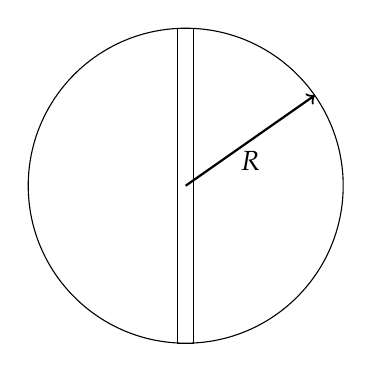
\begin{tikzpicture}
      \draw(0,0) circle(2);
      \draw(-0.1,2) rectangle(0.1,-2);
      \draw[->,thick,rotate=35](0,0)--(2,0) node[midway,below]{$R$};
    \end{tikzpicture}
  \end{center}
  \begin{enumerate}[noitemsep,leftmargin=20pt]
  \item Setting the potential energy of the mass to be zero at the planet's
    center, calculate the mass's potential energy as a function of distance from
    the center of the planet $U(r)$, for values $r<R$. Sketch this potential
    function.
  \item If the mass is dropped from $R$ from the center of the planet, how long
    will it take until it returns to its original position?
  \item If the mass is dropped from $R/2$ from the center of the planet, will
    it require more, or less, or the same amount of time to return to its
    original position compared to if it was dropped from $R$?
  \item If the mass is dropped from $2R$ from the center of the planet, will
    it require more, or less, or the same amount of time to return to its
    original position compared to if it was dropped from $R$?
  \end{enumerate}
  \newpage
\item Two stars of unequal mass orbit each other about their common center of
  mass as shown. The star of mass $M_1$ orbits in a circle of radius $r$, and
  the star of mass $M_2$ orbits in a circle of radius $2r$.
  \begin{center}
    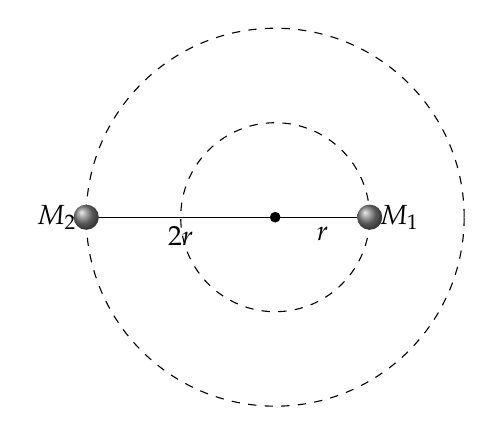
\begin{tikzpicture}[scale=0.8]
      \tikzstyle{balloon}=[ball color=gray];
      \draw[fill=black](0,0) circle(0.075);
      \draw[dashed](0,0) circle(3);
      \draw[dashed](0,0) circle(1.5);
      \draw[->](0,0)--(1.5,0) node[midway,below]{$r$};
      \shade[balloon] (1.5,0) circle (0.2) node[right]{$M_1$};
      \draw[->](0,0)--(-3,0) node[midway,below]{$2r$};
      \shade[balloon] (-3,0) circle (0.2) node[left]{$M_2$};
    \end{tikzpicture}
  \end{center}
  \begin{enumerate}[noitemsep,leftmargin=20pt]
  \item Determine the ratio of masses $M_1/M_2$.
  \item Determine the ratio of the acceleration $a_1$ of $M_1$ to the
    acceleration $a_2$ of $M_2$.
  \item Determine the ratio of the period $T_1$ of $M _1$ to the period $T_2$
    of $M_2$.
  \end{enumerate}

\end{enumerate}
\end{document}
